\documentclass[12pt]{article}

\usepackage{sbc-template}
\usepackage[brazil]{babel}   
\usepackage[utf8]{inputenc}  
\usepackage{url}
\usepackage{amsmath,amssymb,amsfonts}
\usepackage{algorithmic}
\usepackage{graphicx}
\usepackage{textcomp}
\usepackage{subcaption}
\usepackage{hyperref}
\usepackage{xcolor}
\usepackage{cite}
\usepackage[colorinlistoftodos,prependcaption,textsize=tiny]{todonotes}
\usepackage{booktabs}
\usepackage{float}

\def\BibTeX{{\rm B\kern-.05em{\sc i\kern-.025em b}\kern-.08em
    T\kern-.1667em\lower.7ex\hbox{E}\kern-.125emX}}
\begin{document}

\sloppy

\title{Impacto do \textit{Prefetcher} na Precisão de\\ Simulações de Arquiteturas Paralelas\footnote{Este trabalho foi parcialmente financiado pelo projeto Petrobras 2016/00133-9, pela CAPES, CNPq e FAPERGS.}}

\author{Valéria S. Girelli\inst{1}, Francis B. Moreira\inst{1}, Matheus S. Serpa\inst{1} e Philippe O. A. Navaux\inst{1} }


\address{Instituto de Informática -- Universidade Federal do Rio Grande do Sul (UFRGS)\\
	Caixa Postal 15.064 -- 91.501-970, Porto Alegre -- RS -- Brasil
\email{\{vsgirelli, fbmoreira, msserpa, navaux\}@inf.ufrgs.br}
}

\maketitle



\begin{abstract}
In computer architecture research, the use of simulators is predominant, with a wide variety of approaches and implementations. 
However, validation studies lack a detailed analysis of parallel architecture simulators that support High Performance Computing (HPC) workloads. 
This study aims to analyze the impact of the prefetcher in the parallel simulation accuracy of ZSim, a parallel architecture simulator.
We could observe that, due to the lack of a prefetcher model, the memory hierarchy statistics show inaccurate behavior, with error rates reaching 2,600\%.
\end{abstract}

\vspace{-2mm}
\begin{resumo} 
Em arquitetura de computadores, o uso de simuladores é predominante em todos os grupos de pesquisa, com uma ampla variedade de abordagens e implementações.% de simuladores modernos. 
No entanto, falta na literatura uma análise detalhada de simuladores de arquiteturas paralelas que suportem workloads de Computação de Alto Desempenho (High Performance Computing - HPC). %navaux diria pra usar HPC provavelmente 
Este trabalho busca analisar o impacto do prefetcher na precisão da simulação paralela realizada pelo ZSim, um simulador de arquiteturas paralelas.
Observamos que, devido à falta de modelagem de prefetcher, as estatísticas da hierarquia de memória apresentam comportamentos imprecisos, com erros de até 2.600\%. 

%Os ganhos da maioria de técnicas de cache testadas sem prefetch são anulados para os benchmarks testados.
\end{resumo}
% a intro fala tudo que tem sobre os simuladores no abstract. Cortar coisas do abstract e deixar só na intro:
% têm grande importância no desenvolvimento de novas ideias de implementação e na análise de suas consequências na performance de um sistema. A utilização de simuladores leva a uma variedade de abordagens e implementações que impactam diretamente nos resultados observados.

\vspace{-1mm}
\section{Introdução}

\vspace{-1mm}
Na pesquisa de arquiteturas de computadores, a complexidade e alto custo de manufatura inviabilizam a realização de experimentos e análises com implementações físicas. 
Simuladores de arquitetura de processadores são amplamente utilizados no desenvolvimento e análise de novas ideias arquiteturais.
%Portanto, a análise de problemas arquiteturais e o desenvolvimento de ideias novas e suas consequências na performance de uma arquitetura são avaliadas através do uso de modelos e simuladores. 
Deste modo, simulação é considerada a principal forma de se implementar e avaliar uma nova ideia neste campo de pesquisa~\mbox{\cite{demme2014overcoming}}.

\vspace{-2mm}
Em um sistema de computação de alto desempenho (\textit{High Performance Computing - HPC}), encontram-se inúmeros outros problemas além dos já intrínsecos à arquitetura. 
Desenvolver e analisar novas implementações arquiteturais que minimizem o impacto de problemas decorrentes do paralelismo requer simuladores de arquiteturas \textit{multicore} e \textit{manycore} que trabalhem com \textit{workloads} paralelos e suas particularidades.
Por exemplo, sistemas com dezenas de \textit{cores} evidenciam problemas como a interferência entre diferentes \textit{threads} e os custos de comunicação entre elas. 
A interação entre \textit{threads} se dá principalmente por meio de memória compartilhada, com várias \textit{threads} acessando os mesmos endereços de memória.
Com isso, é necessário manter a coerência dos dados na hierarquia de memória por meio de protocolos de coerência de \textit{cache}, que garantem a consistência dos dados por meio de um conjunto de requisições e mensagens.

\vspace{-2mm}
A inserção de \textit{prefetching} em uma arquitetura traz uma nova complexidade ao comportamento da hierarquia de memória no processador.
\textit{Prefetchers} detectam padrões de acesso de cada \textit{core} e geram acessos à memória de forma especulativa, a fim de mitigar o efeito da latência dos acessos aos dados em memória.
Com isso, simulações devem considerar informações muitas vezes descartadas por protocolos de coerência de \textit{cache}, como conteúdos de linha de \textit{cache}\cite{huberty2018content}, valores de registradores\cite{nesbit2004data}, ou endereços físicos~\cite{bakhshalipour2019evaluation}.
 

%Dentre os vários simuladores encontrados na literatura, deseja-se um que seja preciso, rápido, e de fácil extensão e compreensão. Em geral, estes parâmetros não andam juntos~\cite{eeckhout2010evaluation}; por exemplo, simuladores precisos necessitam de detalhamento nas características arquiteturais implementadas, o que aumenta a complexidade do código e diminui a velocidade de simulação. 
%Consequentemente, simular arquiteturas paralelas é ainda mais custoso, tanto do ponto de vista da complexidade da implementação quanto do ponto de vista de tempo de simulação. 
%Diante disso, os diferentes simuladores existentes optam por priorizar subconjuntos de características, aplicando diferentes abordagens de simulação. 

\vspace{-2mm}
Neste trabalho, utilizamos o ZSim~\mbox{\cite{sanchez2013zsim}}, um simulador de arquiteturas paralelas que implementa uma metodologia de simulação também paralela, diminuindo o tempo de simulação.
%O ZSim utiliza a ferramenta Pin\footnote{https://software.intel.com/en-us/articles/pin-a-dynamic-binary-instrumentation-tool} para instrumentação da aplicação, tirando proveito da tradução binária em tempo de execução para simular o comportamento da aplicação (\textit{execution-driven}). 
%Analisando a forma como a simulação paralela é implementada pelo ZSim, observamos que o erro relativo da simulação pode aumentar conforme aumenta-se o paralelismo sendo simulado.
Devido à forma como o ZSim mantém a precisão na \textbf{ordem} da simulação de acessos à \textit{cache}, isso impossibilita a simulação correta de \textit{prefetchers}.
Deste modo, neste trabalho buscamos analisar como a falta de um modelo de \textit{prefetcher} impacta a precisão da simulação do ZSim conforme varia-se o número de threads e quais as consequências desse impacto.%\todo{Texto de contribuições? Seria uma boa, ver espaço}

%Por exemplo, para escrever em uma posição de memória, é necessária uma requisição de exclusividade sobre a linha de \textit{cache} correspondente e mensagens de invalidação para as demais cópias presentes na hierarquia de \textit{cache}.
%Devido à isso, observamos que o número de acessos simulados pelo ZSim à \emph{cache} de último nível é muito alto em relação à execução real.
%\todo{ver com francis}

\vspace{-2mm}
As próximas seções estão organizadas da seguinte forma. 
Na Seção \ref{related} detalhamos os trabalhos relacionados. Na seção \ref{motivacao} apresentamos o conceito de \textit{prefetching} e a implementação do simulador utilizado. A Seção \ref{metodologia} apresenta as configurações dos experimentos e simulações. 
A Seção \ref{resultados} exibe e discute os experimentos realizados, e por fim a Seção \ref{conclusao} apresenta as conclusões e trabalhos futuros.

\vspace{-2mm}
\section{Trabalhos Relacionados}\label{related}

Devido à propriedade intelectual e à falta de informação explícita que empresas de \mbox{\textit{hardware}} empregam para evitar competição, é difícil obter uma simulação ideal que apresente de forma correta todas as características do processador e de sua arquitetura.
Portanto, procura-se em um simulador um erro relativo baixo e sensibilidade em relação ao que se deseja testar~\cite{eeckhout2010computer}. 
Por exemplo, um simulador que não sofre perda de desempenho ao reduzirmos a quantidade de \textit{cache} para programas que exigem muita memória não modela a \textit{cache} corretamente ou sofre de gargalos em outras partes do modelo, impedindo que a sensibilidade da aplicação aos acessos à memória transpareça.
\emph{Microbenchmarks} podem ser usados para diminuir o erro em estruturas básicas da arquitetura, e como forma de engenharia reversa de características arquiteturais ~\cite{fog2012microarchitecture}.


\vspace{-2mm}
Em ~\cite{desikan2001measuring}, estudou-se a dificuldade de se obter informações precisas e a relevância disto ao validar o simulador SimpleScalar~\cite{austin2002simplescalar}.
Ao obter mais informações sobre o modelo do processador Alpha 21264, os autores conseguiram reduzir o erro experimental de \textit{microbenchmarks} de 19,5\% para 2\%. 
Já com a carga de trabalho SPEC-CPU 2000, o erro experimental médio foi de 36,7\% para 18,2\%.
Os autores então mostraram como os recursos achados geram gargalos em partes diferentes do sistema do que previamente modelado em vários artigos, invalidando ideias que apresentavam ganhos de performance onde não havia gargalo.

\vspace{-2mm}
Desde então, vários simuladores foram criados com a intenção de propor juntamente uma validação.
Dentre eles, o ZSim foi selecionado para um estudo aprofundado devido à sua velocidade e precisão, características apresentadas tanto em sua validação~\cite{ZSim2016validation} quanto no estudo de ~\cite{akram2019survey}.
Na pesquisa de Akram, os simuladores gem5~\cite{binkert2011gem5}, Multi2Sim~\mbox{\cite{ubal2012multi2sim}}, MARSSx86~\cite{patel2011marss}, PTLsim~\cite{yourst2007ptlsim}, Sniper~\cite{carlson2011sniper}, e ZSim~\cite{sanchez2013zsim} são avaliados. 
Após uma caracterização minuciosa dos simuladores, foram executadas cargas de trabalho de um \textit{core} e de múltiplos \textit{cores} em cada simulador. 
Os resultados foram comparados com a arquitetura Haswell da Intel~\cite{hammarlund2014haswell}. 
Os autores então destacaram as fontes de erro dos simuladores, sua sensitividade a diferentes parâmetros da arquitetura, e seu erro relativo.
Assim, concluíram que a falta de validação de certos simuladores, por mais populares que sejam (e.g. gem5), leva a uma precisão baixa e pode tornar experimentos inválidos devido às conclusões errôneas.
No entanto, o trabalho de Akram não utiliza cargas de trabalho \textit{multi-thread} para verificar o erro relativo ao número de \emph{threads}.


%Mesmo simuladores mais precisos e rápidos, como ZSim e Sniper, são limitados pois não podem ser facilmente estendidos e não simulam o sistema operacional, o que leva a decisões difíceis na hora de escolher um simulador.
%Esta é a principal causa do grande número de simuladores existentes: nenhum simulador é exatamente o desejado pelo pesquisador, e para atender suas demandas é necessário escrever um novo~\mbox{\cite{sanchez2013zsim,alves2015sinuca}}. 

\vspace{-3mm}
\section{Motivação}\label{motivacao}
\vspace{-1mm}
Nesta Seção, apresentamos o conceito de \textit{prefetching} e a abordagem empregada pelo ZSim em sua simulação paralela.

\vspace{-2mm}
\subsection{Prefetcher}

\begin{figure*}[b!]
    \centering
        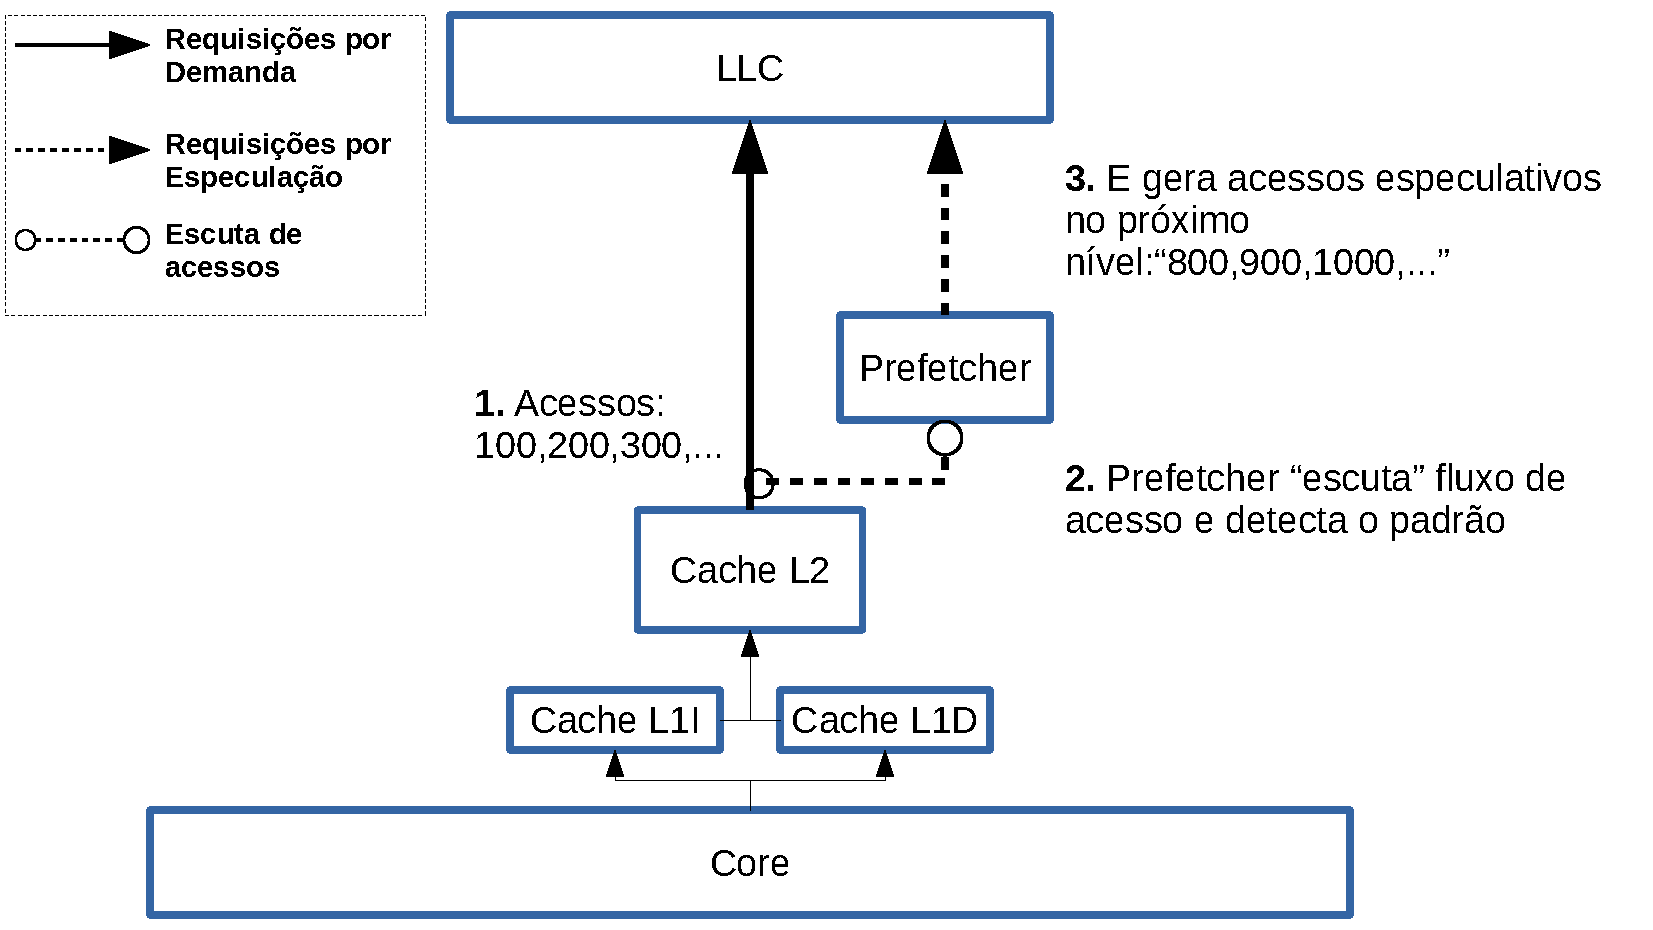
\includegraphics[width=\textwidth]{figures/figpref.pdf}
  \caption{Abstração do funcionamento de um \emph{prefetcher}.}
  \label{fig:prefetcher}
\end{figure*}

\vspace{-1mm}
A memória disponível para um processador está organizada em diferentes níveis. 
Níveis privados e mais próximos do processador possuem menor capacidade de armazenamento e acesso de dados mais eficiente.
Quando um processador faz uma requisição à memória, esta requisição é feita ao primeiro nível da hierarquia de memória interna do processador, a memória \textit{cache} de dados de primeiro nível (L1).
Esta memória é relativamente pequena (32~\emph{kilobytes}) e de baixa latência~(4~ciclos do processador).
Caso uma cópia do dado requisitado não se encontre na \textit{cache} de dados L1, a mesma encaminha a requisição ao próximo nível de memória \emph{cache}, que repete o mesmo procedimento.
O último nível de memória \textit{cache} (\textit{Last Level Cache - LLC}), por sua vez, encaminha a requisição para a memória principal.
Caso esta não tenha o dado, ocorre uma falta de página e a página precisa ser buscada em um dispositivo armazenamento secundário.
Desse modo, deseja-se que os níveis de \textit{cache} mais próximos do processador possuam os dados necessários para o momento da execução de cada requisição à memória.


\vspace{-2mm}
Para reduzir a latência de acesso aos dados, criou-se o \textit{prefetcher}.
Com base no padrão dos acessos gerados pelo processador, especula-se qual seria o próximo endereço a ser requisitado e busca-se o bloco de dados antecipadamente.
Deste modo, quando o bloco de dados for requisitado, o mesmo já estará em \emph{caches} mais próximas ao processador.
Alguns padrões observados são o \emph{stride}~\cite{chen1995effective} e o \emph{stream}~\mbox{\cite{le2007ibm}}.

\vspace{-2mm}
A Figura \ref{fig:prefetcher} exibe um exemplo do funcionamento do \textit{prefetcher} identificando um padrão de acesso \textit{strided}.
O segundo nível de \textit{cache} (L2) encaminha requisições para a LLC (indicado na Figura \ref{fig:prefetcher} como o evento \textbf{1}).
O \textit{prefetcher}, por sua vez, intercepta essas requisições (\textbf{2}) e identifica o padrão de acesso sendo gerado.
Com base no padrão identificado, acessos especulativos à LLC são realizados (\textbf{3}).
Estes acessos são vistos como requisições normais realizadas pela L2, então a LLC encaminha esses dados à L2.
Assim, quando os dados requisitados por \textit{prefetch} forem necessários, eles já estarão em níveis de \textit{cache} mais próximos do processador.
\textit{Prefetchers} são predominantes em arquiteturas atuais como uma das formas de mitigar o gargalo de acesso à memória principal~\mbox{\cite{bakhshalipour2019bingo}}.


%\todo{citar papers que falam sobre a utilidade do prefetch, quanto de desempenho pode-se alcançar a mais, etc}
\vspace{-2mm}
\subsection{ZSim}

O ZSim implementa a simulação em um método de duas fases chamadas \mbox{\textit{Bound} e \emph{Weave}}. 
Na fase \textit{Bound} são simulados alguns milhares de ciclos, ignorando-se contenção e usando latências mínimas para todos acessos à memória.
Registra-se um traço dos acessos à memória, incluindo quais \textit{caches} foram acessadas, invalidações, etc.
Na fase \textit{Weave} é feita a simulação paralela orientada aos eventos do intervalo registrado para determinar as latências reais dos acessos.
Como as interações entre os acessos à memória já foram identificadas na primeira fase, esta simulação de \emph{timing} dos acessos pode ser feita de forma eficiente, mantendo-se uma alta precisão.

\vspace{-2mm}
Os autores observaram que, em um intervalo de alguns milhares de ciclos, a maior parte dos acessos concorrentes entre diferentes \textit{cores} acontece a linhas de \textit{cache} não relacionadas. 
Portanto, simular estes acessos não relacionados fora de ordem ignorando contenções e, posteriormente, simulá-los em ordem respeitando restrições temporais, é equivalente a simulá-los completamente em ordem.
%\todo{será? em 1 set temos X linhas. proc A quer 1 linha desse set mas não está ali no momento, proc B quer 1 linha desse set e está ali. Se proc A chega antes e a cache chuta a linha q proc B queria para colocar a linha q proc A quer, a ordem importa, não? Os autores do ZSim dizem que a maior parte dos acessos não vão ter nenhuma relação, mas assumem q vão ocorrer erros qd esse tipo de coisa acontecer. Acho q estás com 1 percepção errada, pois o teu texto pode levar pessoas a acreditarem em outras coisas} 


%Portanto, independente da ordem em que os acessos são tratados, nada muda na coerência do sistema de \textit{cache}.
%Não são necessárias requisições de exclusividade, de invalidação, e de atualização de cópias. 
%\todo{frase pode confundir pessoas, cortei fora, ver todo acima. não é isso que acontece no zsim. o texto abaixo tb só vê a perspectiva de acessos a mesma linha, mas não é só esse o caso que os autores do zsim querem dizer com acessos "relacionados" a uma linha}

% ou geram \textit{prefetches} devido à sua ordem
\vspace{-2mm}
No entanto, quando acessos estão relacionados, \emph{i.e.}, acessam a mesma linha de \mbox{\textit{cache}}, é necessário manter a coerência das diferentes cópias do dado nos diferentes \mbox{\textit{cores}}.
Um exemplo disso é quando um \textit{core} demanda acesso exclusivo a uma linha de \mbox{\textit{cache}} compartilhada para realizar uma escrita na mesma, fazendo com que o protocolo de coerência de \textit{cache} invalide as demais cópias da linha na hierarquia de \textit{cache} do sistema. 
%O conjunto de requisições e mensagens necessárias para se invalidar as demais cópias da linha para obtê-la de forma exclusiva é conhecido como \textit{Request for Ownership - RFO}. 
No entanto, por serem consideradas raras, a \textbf{ordem} dessas interações não é modelada pelo ZSim, o que pode resultar na alteração do caminho desses dados na hierarquia de \textit{cache}.
A alteração do caminho dos dados na \textit{cache} pode impactar no número de ciclos, de \textit{misses}, e de mensagens de coerência observados na simulação.
Além disso, a geração e os caminhos das requisições feitas por \textit{prefetches} também podem sofrer alterações, o que impede a modelagem de \textit{prefetcher} neste modelo.


\vspace{-2mm}
Em sua validação, o ZSim utiliza o \emph{benchmark} PARSEC~\cite{bienia2008parsec} e mostra apenas que o \emph{speed-up} é próximo ao obtido com execuções reais ao variar o número de \emph{threads}.
Deste modo, uma vez que o \textit{prefetcher} não é simulado, buscamos avaliar a precisão do método de simulação \textit{Bound and Weave} utilizado para simular paralelamente múltiplas estruturas e \textit{threads}.

\vspace{-2mm}

\section{Ambiente de Experimentos}\label{metodologia}

Nesta Seção são especificadas as configurações dos ambientes usados para a realização de nossos experimentos.
%\fi % fim do comentário
\vspace{-2mm}
\subsection{Configurações de Processador}

%Na Tabela~\ref{tablehb} estão enumeradas as configurações utilizadas para os testes.
A ferramenta \emph{perf}~\cite{de2010new} foi usada para obter os valores dos contadores de \textit{hardware} para todas as execuções reais.
Em cada execução real avalia-se um contador, evitando-se assim agregações ou aproximações da ferramenta que ocorrem ao avaliar múltiplas estatísticas na mesma execução.  
O desempenho e estatísticas da execução real foram avaliados através de 10 execuções de cada estatística, para cada \emph{benchmark}, em máquinas \emph{draco}, todas idênticas, pertencentes ao \emph{cluster} do Parque Computacional de Alto Desempenho (PCAD)\footnote{http://gppd-hpc.inf.ufrgs.br/}, pertencente ao GPPD - Grupo de Processamento Paralelo e Distribuído.
Para as simulações foram utilizadas configurações que se aproximam da máquina real, uma Intel(R) Xeon(R) CPU E5-2640 v2, de arquitetura Ivy Bridge~\cite{james2012intel}, respeitando-se as limitações do simulador.
Cada simulação foi executada apenas uma vez, e todas as estatísticas são extraídas desta mesma simulação.

\vspace{-2mm}
Neste artigo exibimos uma seleção de estatísticas, onde são ilustrados problemas na modelagem de hierarquia de memória do ZSim.
Escolhemos as estatísticas de ciclos de execução, acessos à memória \emph{cache} de dados L1, e acessos ao último nível de memória \emph{cache}.
%Todas as estatísticas são ilustradas com os valores agregados entre todas as\emph{threads}.
As estatísticas de ciclos ilustram o maior número de ciclos levado pelas \emph{threads} paralelas, efetivamente representando o tempo que a aplicação levou para executar.
As estatísticas de acessos à memória \emph{cache} L1 representam uma média entre as \emph{caches} de todas as \emph{threads}, onde podemos notar as estruturas de dados sendo divididas entre as \emph{threads} conforme aumentamos o paralelismo da aplicação.
O último nível de \textit{cache} é dividido em 8 bancos (um por \textit{core}) conectados por um anel bidirecional.
Um \textit{core} acessa todos os bancos, pois os endereços de memória são divididos entre os bancos por meio de uma função de \textit{hash}.
Assim, as estatísticas da LLC contam os acessos a todos os bancos.
O desvio padrão dos dados relativos às 10 execuções reais das aplicações não é apresentado nos gráficos por ser menor que 1\%. %i.e. negligível,insignificante. Usaste 7 palavras onde cabe 1.

%\iffalse % comentário
\begin{table}[h]
    \centering
    \footnotesize
    \caption{Configurações do processador real e do processador simulado.}
    \label{tablehb}
    \renewcommand{\tabcolsep}{1pt}
   % \newcolumntype{L}[1]{>{\raggedright\let\newline\\\arraybackslash\hspace{0pt}}m{#1}}
    \begin{tabular}{{@{\hspace{0.0cm}} l @{\hspace{0.1cm}} @{\hspace{0.1cm}} c @{\hspace{0.1cm}} @{\hspace{0.1cm}} c @{\hspace{0.1cm}} @{\hspace{0.1cm}} c @{\hspace{0.1cm}} @{\hspace{0.1cm}}}}
    \toprule
    & \bfseries Real &\bfseries ZSim  \\
    \midrule
    Frequência do Processador & 2 - 2.5Ghz & 2Ghz \\

    Número de \emph{Cores} & 8 & 8  \\

    Número de Estágios & 18 & 14  \\

%    Busca de Instruções & 16B & 16B  \\
    
%    Fila de Instruções & 18 & \textbf{NA} \\
    
%    Decodificação Paralela & até 5 uops & até 5 uops \\
    
%    Buffer de Decodificação & 56 & 28 \\
    
%    \emph{cache} de uops & 1536 uops & \textbf{NA} \\ 
    
%    Renomeação & 4 uops & 4 uops \\
    
%    Estações de Reserva & 54 & 36 \\
    
%    Execução  & até 6 uops & até 5 uops \\
    
%    Buffer de Reordenamento & 168 & 128 \\
    
%    Buffer de Leitura & 32 & 32 \\
    
%    Buffer de Escrita & 16 & 32 \\
    
%    Graduação Paralela & 4 & 5 \\
   
 %   \midrule
 %   Preditor de Desvios & Tournament  & 2-level PAg \\
    
 %   Penalidade & 15-20 & 17 \\
    
    \midrule
    Tamanho da Linha de \emph{cache} & 64~B & 64~B \\
    
	\emph{Cache} de Dados L1 & 8- \emph{way} 32KB & 8- \emph{way} 32KB \\
	
	Latência & 4 & 4 \\
    \midrule
    
    \emph{Cache} de Instruções L1 & 8- \emph{way} 32KB & 8- \emph{way} 32KB \\
	
	Latência & 4 & 3 \\
    \midrule
    
	\emph{Cache} Unificada L2 & 8- \emph{way} 256KB & 8- \emph{way} 256KB \\
    
    Latência & ca. 11 & 12 \\
    \midrule
    
    \emph{Cache} de Último Nível L3 & 20- \emph{way} 20MB & 16- \emph{way} 16MB \\
    
    Latência & ca. 28 & 30 \\
    \midrule
    \textit{Prefetchers} & \emph{L1 IP Stride} & \\
                & \emph{Adjacent Line prefetcher} & \\
                & \textit{L2 DCU Stream prefetcher} & \\
    \bottomrule
    \end{tabular}
\end{table}
%\fi % fim comentário

\vspace{-2mm}
\subsection{Configurações de \emph{benchmark}}
Para a avaliação de escalabilidade do erro relativo ao número de \emph{threads}, foi usado o \emph{benchmark} \emph{Numerical Aerodynamic Simulation Parallel} \emph{Benchmarks} (NPB)~\mbox{\cite{jin1999openmp}}.
Este \emph{benchmark} é composto por dez aplicações paralelas, das quais nove foram usadas.
As aplicações utilizadas neste trabalho são:


%\iffalse % comentário
\vspace{-1mm}
\begin{itemize}

\item \textbf{CG}: \emph{Conjugate Gradient} utiliza um método de gradiente conjugado para aproximar o valor do menor autovalor de uma matriz simétrica positiva definida, grande e esparsa. Este \emph{kernel} testa comunicação de longa distância irregular, empregando multiplicação de matriz por vetor sem estrutura.
\item \textbf{EP}: \emph{Embarrassingly Parallel} resolve o problema de gerar pares de gaussianas e tabular seus valores em quadrados \emph{annuli} sucessivos. Ao contrário do resto da lista, este \emph{kernel} praticamente não possui comunicação, estressando apenas o desempenho de operações de ponto flutuante.
\item \textbf{FT}: \emph{Fourier Transform} resolve o problema da transformada de Fourier tridimensional de forma paralela usando o algoritmo de transformada rápida de Fourier (FFT). Testa rigorosamente a comunicação de alta distância, ocorrendo comunicação de todos \emph{cores} com todos \emph{cores}. 
\item \textbf{IS}: \emph{Integer Sort} resolve o problema de ordenar inteiros usando \emph{bucket sort}. Possui acessos randômicos à memória, e testa tanto o desempenho de operações com inteiros quanto a comunicação.
\item \textbf{MG}: \emph{Multigrid} resolve um problema simplificado de cálculo \emph{multigrid}, testando comunicações de curta e longa distâncias. Requer comunicação de longa distância altamente estruturada.
\item \textbf{UA}: \emph{Unstructured Adaptive Mesh} resolve um problema estilizado de transferência de calor em um domínio cúbico, discretizado em uma malha sem estrutura refinada adaptativamente.
\item \textbf{BT}: \emph{Block Tridiagonal} resolve um problema sintético de CFD com múltiplos sistemas de equações de blocos tridiagonais 5x5 com diagonais não-dominantes. Tem paralelismo mais limitado que os outros CFD (LU e SP).
\item \textbf{LU}: \emph{Lower Upper Gauss Seidel Solver} resolve um problema sintético de CFD ao resolver um sistema de equações lineares triangulares esparsas, com blocos de 5x5. Envolve dependências de dados globais, com várias comunicações curtas.
\item \textbf{SP}: \emph{Scalar Pentadiagonal} resolve sistemas de equações escalares pentadiagonais com diagonais não-dominantes. 
Assim como o LU, envolve dependências de dados globais, mas com comunicações mais infrequentes e mais longas.
\end{itemize}

\vspace{-1mm}
A aplicação \textbf{DC} ("Data Cube") não foi usado devido à grande utilização de I/O, o qual não é modelado pelos simuladores.

%\newpage
\vspace{-2mm}
\section{Análise de Comportamento da Hierarquia de Memória}\label{resultados}

\begin{figure*}[t]
  \hspace{+25mm}
  \begin{subfigure}{0.33\textwidth}
    \centering
        
\includegraphics[width=10cm,height=0.7cm]{figures/legend.png}
    \label{fig:leg}
  \end{subfigure}
  \vspace{-5mm}

  \begin{subfigure}{0.33\textwidth}
    \centering
    \vspace{-4mm}
        \includegraphics[width=4.7cm,height=4.9cm]{figures/ftcy.png}
    \caption{Número de ciclos}
    \label{fig:ftcycles}
  \end{subfigure}%
  \begin{subfigure}{0.33\textwidth}
    \centering	
        \includegraphics[width=4.7cm,height=5cm]{figures/ftl1.png}
    \caption{Número de acessos à \textit{cache} L1 de dados}
    \label{fig:ftl1}
  \end{subfigure}%
  \begin{subfigure}{0.33\textwidth}
    \centering	
        \includegraphics[width=4.7cm,height=5cm]{figures/ftllc.png}
    \caption{Número de acessos à \textit{cache} LLC}
    \label{fig:ftllc}
  \end{subfigure}
  
  \caption{Comparações entre execução real com \textit{prefetch}, execução real sem \textit{prefetch} e simulação da aplicação FT.}
  \label{ref:ft}
\end{figure*}

\begin{figure*}[t!]
  \hspace{+25mm}
  \begin{subfigure}{0.33\textwidth}
    \centering
        
\includegraphics[width=10cm,height=0.7cm]{figures/legend.png}
    \label{fig:epleg}
  \end{subfigure}
  \vspace{-5mm}

  \begin{subfigure}{0.33\textwidth}
    \centering
    \vspace{-4mm}
        \includegraphics[width=4.7cm,height=4.9cm]{figures/epcy.png}
    \caption{Número de ciclos}
    \label{fig:epcycles}
  \end{subfigure}%
  \begin{subfigure}{0.33\textwidth}
    \centering	
        \includegraphics[width=4.7cm,height=5cm]{figures/epl1.png}
    \caption{Número de acessos à \textit{cache} L1 de dados}
    \label{fig:epl1}
  \end{subfigure}%
  \begin{subfigure}{0.33\textwidth}
    \centering	
        \includegraphics[width=4.7cm,height=5cm]{figures/epllc.png}
    \caption{Número de acessos à \textit{cache} LLC}
    \label{fig:epllc}
  \end{subfigure}
  
  \caption{Comparações entre execução real com \textit{prefetch}, execução real sem \textit{prefetch} e simulação da aplicação EP.}
  \label{ref:ep}
\end{figure*}


%Quando um \textit{core} precisa de acesso exclusivo a uma linha de \emph{cache} compartilhada para realizar uma escrita na mesma, as demais cópias da linha devem ser invalidadas na hierarquia de \emph{cache} do sistema. 
%O conjunto de requisições e mensagens necessárias para se invalidar as demais cópias da linha para obtê-la de forma exclusiva é conhecido como \textit{Request for Ownership - RFO}. 
%Sabe-se que o ZSim não modela a \textbf{ordem} de execução de acessos desse tipo, ou seja, uma \emph{cache} pode ter requisitado uma linha como exclusiva antes de outra \emph{cache}, mas o ZSim não garante que essas requisições sejam de fato simuladas em ordem. 
%Desse modo, a ordem em que os RFOs são simulados altera a ordem das mensagens de invalidação no sistema de \emph{cache}, o que pode impactar nas latências dos acessos subsequentes e na quantidade de misses observados.
%Portanto, esperávamos encontrar inconsistências com relação à quantidade de ciclos e misses simulados se comparado à execução real.

\vspace{-1mm}
Uma vez que o ZSim não simula o sistema de \textit{prefetching}, poderiam ocorrer alterações no número de ciclos, \textit{misses}, e acessos à LLC.
Analisamos, portanto, o número de ciclos e de acessos à \textit{cache} de dados e à LLC observados na simulação e na execução real com e sem a atuação do \textit{prefetch}. 

\vspace{-2mm}
A Figura \ref{ref:ft} apresenta o comportamento observado na aplicação FT.
A Figura \ref{fig:ftcycles} mostra o número de ciclos da aplicação.
Podemos observar que o erro relativo do ZSim em relação ao \emph{speed-up} da aplicação é bom, pois acompanha a tendência da execução real, comportamento observado em todos os \textit{benchmarks} analisados.
A Figura \ref{fig:ftl1} apresenta o número de acessos à memória \textit{cache} L1 de dados da aplicação.
Observa-se que, apesar de também seguir a mesma tendência das execuções reais, apresenta uma diferença grande no número de acessos observados.
%Pode-se observar que o número de acessos à \textit{cache} L1 é muito inferior na simulação se comparado às execuções reais.
%Enquanto os acessos à L1 são sempre menores na simulação, um comportamento contrário é observado com relação aos acessos ao último nível de \textit{cache}.
Uma grande diferença também é observada no número de acessos ao último nível de \textit{cache}, como exibido na Figura \ref{fig:ftllc}.
No entanto, os acessos à LLC seguem uma tendência contrária à das execuções reais, decrescendo na simulação.




\begin{figure*}[t!]
  \hspace{+25mm}
  \begin{subfigure}{0.33\textwidth}
    \centering
        
\includegraphics[width=10cm,height=0.7cm]{figures/legend.png}
    \label{fig:isleg}
  \end{subfigure}
  \vspace{-5mm}

  \begin{subfigure}{0.33\textwidth}
    \centering
    \vspace{-4mm}
        \includegraphics[width=4.7cm,height=4.9cm]{figures/iscy.png}
    \caption{Número de ciclos}
    \label{fig:iscycles}
  \end{subfigure}%
  \begin{subfigure}{0.33\textwidth}
    \centering	
        \includegraphics[width=4.7cm,height=5cm]{figures/isl1.png}
    \caption{Número de acessos à \textit{cache} L1 de dados}
    \label{fig:isl1}
  \end{subfigure}%
  \begin{subfigure}{0.33\textwidth}
    \centering	
        \includegraphics[width=4.7cm,height=5cm]{figures/isllc.png}
    \caption{Número de acessos à \textit{cache} LLC}
    \label{fig:isllc}
  \end{subfigure}
  
  \caption{Comparações entre execução real com \textit{prefetch}, execução real sem \textit{prefetch} e simulação da aplicação IS.}
  \label{ref:is}
\end{figure*}

\begin{figure*}[t!]
  \hspace{+25mm}
  \begin{subfigure}{0.33\textwidth}
    \centering
        
\includegraphics[width=10cm,height=0.7cm]{figures/legend.png}
    \label{fig:mgleg}
  \end{subfigure}
  \vspace{-5mm}

  \begin{subfigure}{0.33\textwidth}
    \centering
    \vspace{-4mm}
        \includegraphics[width=4.7cm,height=4.9cm]{figures/mgcy.png}
    \caption{Número de ciclos}
    \label{fig:mgcycles}
  \end{subfigure}%
  \begin{subfigure}{0.33\textwidth}
    \centering	
        \includegraphics[width=4.7cm,height=5cm]{figures/mgl1.png}
    \caption{Número de acessos à \textit{cache} LLC}
    \label{fig:mgl1}
  \end{subfigure}%
  \begin{subfigure}{0.33\textwidth}
    \centering	
        \includegraphics[width=4.7cm,height=5cm]{figures/mgllc.png}
    \caption{Número de acessos à \textit{cache} LLC}
    \label{fig:mgllc}
  \end{subfigure}
  
  \caption{Comparações entre execução real com \textit{prefetch}, execução real sem \textit{prefetch} e simulação da aplicação MG.}
  \label{ref:mg}
\end{figure*}

%\vspace{-2mm}
%O comportamento da aplicação SP pode ser observado na Figura \ref{ref:sp}.
%Pode-se observar que o número de acessos à LLC realizados pela simulação é mais coerente se comparado à execução real sem \textit{prefetch}, que não muda o número de acessos ao último nível de \textit{cache}.
%Porém, para uma e duas \emph{threads}, a simulação do ZSim ainda apresenta um aumento significativo nos acessos quando comparada à execução real sem \textit{prefetch}.
\vspace{-2mm}
Na Figura \ref{ref:ep} observamos os resultados obtidos na aplicação EP.
Na Figura \ref{fig:epllc}, que apresenta os acessos à LLC, pode-se ver claramente a falta de modelagem de \textit{prefetcher}.
Comparando-se a execução com \textit{prefetcher} à execução sem \textit{prefetcher}, observa-se que um grande número de acessos à LLC é evitado pelos acessos especulativos realizados pelo \textit{prefetcher}.
Apesar de o simulador seguir as tendências da execução real fielmente, há uma diferença maior que 2.000\% na quantidade de acessos que chegam ao último nível de \textit{cache}.
Comportamento semelhante é observado na aplicação IS, ilustrada na \mbox{Figura \ref{ref:is}}.
Embora nesta aplicação o número absoluto de acessos ao último nível de \textit{cache} seja menor, podemos observar que em todas as execuções que a tendência é de aumento nesta métrica.
Esta mesma tendência ocorre nas aplicações LU, UA e MG.

\begin{figure*}[t!]
  \hspace{+25mm}
  \begin{subfigure}{0.33\textwidth}
    \centering
        
\includegraphics[width=10cm,height=0.7cm]{figures/legend.png}
    \label{fig:btleg}
  \end{subfigure}
  \vspace{-5mm}

  \begin{subfigure}{0.33\textwidth}
    \centering
    \vspace{-4.5mm}
        \includegraphics[width=4.7cm,height=4.9cm]{figures/btcy.png}
    \caption{Número de ciclos}
    \label{fig:btcycles}
  \end{subfigure}%
  \begin{subfigure}{0.33\textwidth}
    \centering	
        \includegraphics[width=4.7cm,height=5cm]{figures/btl1.png}
    \caption{Número de acessos à \textit{cache} L1 de dados}
    \label{fig:btl1}
  \end{subfigure}%
  \begin{subfigure}{0.33\textwidth}
    \centering	
        \includegraphics[width=4.7cm,height=5cm]{figures/btllc.png}
    \caption{Número de acessos à \textit{cache} LLC}
    \label{fig:btllc}
  \end{subfigure}
  
  \caption{Comparações entre execução real com \textit{prefetch}, execução real sem \textit{prefetch} e simulação da aplicação BT.}
  \label{ref:bt}
\end{figure*}

\begin{figure*}[t!]
  \hspace{+25mm}
  \begin{subfigure}{0.33\textwidth}
    \centering
        
\includegraphics[width=10cm,height=0.7cm]{figures/legend.png}
    \label{fig:cgleg}
  \end{subfigure}
  \vspace{-5mm}

  \begin{subfigure}{0.33\textwidth}
    \centering
    \vspace{-4.mm}
        \includegraphics[width=4.7cm,height=4.9cm]{figures/cgcy.png}
    \caption{Número de ciclos}
    \label{fig:cgcycles}
  \end{subfigure}%
  \begin{subfigure}{0.33\textwidth}
    \centering	
        \includegraphics[width=4.7cm,height=5cm]{figures/cgl1.png}
    \caption{Número de acessos à \textit{cache} L1 de dados}
    \label{fig:cgl1}
  \end{subfigure}%
  \begin{subfigure}{0.33\textwidth}
    \centering	
        \includegraphics[width=4.7cm,height=5cm]{figures/cgllc.png}
    \caption{Número de acessos à \textit{cache} LLC}
    \label{fig:cgllc}
  \end{subfigure}
  
  \caption{Comparações entre execução real com \textit{prefetch}, execução real sem \textit{prefetch} e simulação da aplicação CG.}
  \label{ref:cg}
\end{figure*}

\vspace{-2mm}
Na aplicação MG, ilustrada na Figura \ref{ref:mg}, os acessos ao último nível de \textit{cache} da execução real com \textit{prefetch} aumentam tanto que se aproximam de uma execução sem \textit{prefetch}, como visto na Figura \ref{fig:mgllc}. 
Isto pode ocorrer devido a \textit{prefetchers} imprecisos ou aumento na comunicação.
%Tal aumento pode ser observado em todas aplicações usadas.
Além disso, com o crescimento do número de \mbox{\emph{threads}}, a diferença entre os tempos da simulação e da execução real sem \textit{prefetch} diminuem se comparados à execução com \textit{prefetch}.
Dessa forma, o paralelismo explicita a comunicação como gargalo ao aumentar o número de requisições no último nível de \emph{cache}, inutilizando \textit{prefetchers} e limitando o comportamento em todos os casos analisados.
A única aplicação onde isto não ocorre é a EP, na qual a necessidade de memória e comunicação é tão pequena que cabe no último nível de \textit{cache}.
Com isso, observamos pouca diferença entre os ciclos da execução real com \textit{prefetch} ou sem \textit{prefetch} para o EP, como visto na Figura \ref{fig:epllc}.


\iffalse % comentário
\begin{figure*}[b!]
  \hspace{+25mm}
  \begin{subfigure}{0.33\textwidth}
    \centering
        
\includegraphics[width=10cm,height=0.7cm]{figures/legend.png}
    \label{fig:spleg}
  \end{subfigure}
  \vspace{-5mm}

  \begin{subfigure}{0.33\textwidth}
    \centering
    \vspace{-4mm}
        \includegraphics[width=4.7cm,height=4.9cm]{figures/spcy.png}
    \caption{Número de ciclos}
    \label{fig:spcycles}
  \end{subfigure}%
  \begin{subfigure}{0.33\textwidth}
    \centering	
        \includegraphics[width=4.7cm,height=5cm]{figures/spl1.png}
    \caption{Número de acessos à \textit{cache} L1 de dados}
    \label{fig:spl1}
  \end{subfigure}%
  \begin{subfigure}{0.33\textwidth}
    \centering	
        \includegraphics[width=4.7cm,height=5cm]{figures/spllc.png}
    \caption{Número de acessos à \textit{cache} LLC}
    \label{fig:spllc}
  \end{subfigure}
  
  \caption{Comparações entre execução real com \textit{prefetch}, execução real sem \textit{prefetch} e simulação da aplicação SP.}
  \label{ref:sp}
\end{figure*}


\begin{figure*}[b!]
  \hspace{+25mm}
  \begin{subfigure}{0.33\textwidth}
    \centering
        
\includegraphics[width=10cm,height=0.7cm]{figures/legend.png}
    \label{fig:luleg}
  \end{subfigure}
  \vspace{-5mm}

  \begin{subfigure}{0.33\textwidth}
    \centering
    \vspace{-4mm}
        \includegraphics[width=4.7cm,height=4.9cm]{figures/lucy.png}
    \caption{Número de ciclos}
    \label{fig:lucycles}
  \end{subfigure}%
  \begin{subfigure}{0.33\textwidth}
    \centering	
        \includegraphics[width=4.7cm,height=5cm]{figures/lul1.png}
    \caption{Número de acessos à \textit{cache} L1 de dados}
    \label{fig:lul1}
  \end{subfigure}%
  \begin{subfigure}{0.33\textwidth}
    \centering	
        \includegraphics[width=4.7cm,height=5cm]{figures/lullc.png}
    \caption{Número de acessos à \textit{cache} LLC}
    \label{fig:lullc}
  \end{subfigure}
  
  \caption{Comparações entre execução real com \textit{prefetch}, execução real sem \textit{prefetch} e simulação da aplicação LU.}
  \label{ref:lu}
\end{figure*}

\begin{figure*}[t!]
  \hspace{+25mm}
  \begin{subfigure}{0.33\textwidth}
    \centering
        
\includegraphics[width=10cm,height=0.7cm]{figures/legend.png}
    \label{fig:ualeg}
  \end{subfigure}
  \vspace{-5mm}

  \begin{subfigure}{0.33\textwidth}
    \centering
    \vspace{-4mm}
        \includegraphics[width=4.7cm,height=4.9cm]{figures/uacy.png}
    \caption{Número de ciclos}
    \label{fig:uacycles}
  \end{subfigure}%
  \begin{subfigure}{0.33\textwidth}
    \centering	
        \includegraphics[width=4.7cm,height=5cm]{figures/ual1.png}
    \caption{Número de acessos à \textit{cache} L1 de dados}
    \label{fig:ual1}
  \end{subfigure}%
  \begin{subfigure}{0.33\textwidth}
    \centering	
        \includegraphics[width=4.7cm,height=5cm]{figures/uallc.png}
    \caption{Número de acessos à \textit{cache} LLC}
    \label{fig:uallc}
  \end{subfigure}
  
  \caption{Comparações entre execução real com \textit{prefetch}, execução real sem \textit{prefetch} e simulação da aplicação UA.}
  \label{ref:ua}
\end{figure*}

\fi % fim comentáio



%Ao investigarmos os RFOs gerados pela simulação e pela execução real, pode-se observar que, para todas as aplicações (com exceção da aplicação IS, sobre a qual sera discutido adiante), o número de RFOs simulados é sempre muito superior ao número de RFOs executados.
%Apesar de todas as aplicações apresentarem diferenças, chama a atenção o comportamento apresentado pela aplicação EP, como mostra a Figura \ref{ref:ep}. 
%A aplicação, cujo nome sugestivamente é \textit{Embarrassingly Parallel}, possui uma quantidade negligível de comunicação entre as diferentes \textit{threads}. 
%Enquanto na execução real o número de RFOs é próximo a um milhão para qualquer número de \emph{threads}, na simulação este número ultrapassa 60 milhões. 
%

%Analisando as informações de saída da simulação que são providas pelo ZSim, observa-se que a maior quantidade de RFOs é representada por operações de escrita a linhas que não estavam em nenhum nível de \textit{cache}. 
%Com exceção do IS, todos os \textit{benchmarks} analisados apresentaram uma quantidade muito maior de \textit{stores} a linhas que não estão na hierarquia de \textit{cache} do que o observado na execução real.
%Isso indica que há a necessidade de uma investigação mais profunda na forma como o ZSim modela acessos de escrita a dados compartilhados entre \textit{cores}.
%Desta forma, o problema não é simplesmente ocasionado pela não ordenação de acessos concorrentes (comunicação) como suspeitava-se na hipótese inicial.



%Simulação tem muito menos misses de L1, mas muitos mais RFOs na LLC. 
%\todo fbm: falta elaborar isso em algo coerente. lembra que a estatística mostra misses para LOADS, não stores. Ele pode estar fazendo uma montanha de misses de store na L1 q não estamos vendo com as figuras atuais.

%se não houvesse tanto rfo, talvez o número de ciclos da simulação tbm estaria inferior ao da execução real, assim como os l1 misses.
%todo fbm: talvez, mas como mostrar isso? deixe especulações pras conclusões/future work

%IS é a única aplicação em C.
%todo fbm: desenvolve ou corta daqui e dali de cima a referência ao IS




%No que diz respeito à aplicação IS, foi observado um comportamento diferente com relação ao RFOs simulados. A Figura \ref{fig:isllc} mostra que, apesar de os número de RFOs da execução real crescer linearmente, o crescimento dos RFOs simulados não obedece o mesmo comportamento. Uma vez que o IS é a única aplicação dentre os \textit{benchmarks} analisados cujo código fonte é em C, futuras análises devem ser realizadas para que se possa compreender se a linguagem tem algum impacto nos resultados. 




%\iffalse % comentário



\vspace{-2mm}
Nas aplicações restantes podemos observar comportamentos anômalos.
Na aplicação BT, ilustrada na Figura \ref{ref:bt}, observamos um comportamento similar ao notado até agora para ciclos e acessos à \textit{cache} L1.
Porém, a simulação do ZSim apresenta comportamento errático com relação aos acessos à LLC com uma e duas \emph{threads}. Observa-se na Figura \ref{fig:btllc} que o número de acessos ao último nível de \textit{cache} é muito maior que em ambas as execuções reais.
Com quatro e oito \emph{threads} o comportamento volta ao normal.
A reexecução da simulação foi feita, e este comportamento se mantém, o que indica algum problema específico na interação do simulador com este \textit{benchmark}. %\todo{future work}

\vspace{-2mm}
Na aplicação CG, ilustrada na Figura \ref{ref:cg}, a execução real sem \textit{prefetch} com uma \emph{thread} apresenta um número muito elevado de acessos ao último nível de \textit{cache}.
O desvio padrão observado é menor do que 1\%, o que inviabiliza uma possível variância nos experimentos como explicação para tal comportamento.
Curiosamente, a simulação do ZSim não segue o comportamento da máquina real sem \textit{prefetch} nestes acessos, mas se aproxima no valor de ciclos. 
%\todo{future work}


\vspace{-2mm}
Portanto, é possível constatar que, para todos os \textit{benchmarks} analisados, o número de ciclos simulados é sempre maior do que nas execuções reais com \textit{prefetcher}. 
No que diz respeito aos acessos à \textit{cache} de dados, o número observado na simulação é sempre menor.
Já as estatísticas de acesso à LLC têm comportamento errático, resultado de imprecisão na modelagem da hierarquia de \textit{cache}.




%\fi % fim comentáio
\vspace{-2mm}
A Tabela \ref{table:resumo} ilustra um resumo da diferença existente entre a simulação e a execução real com \textit{prefetch} no que diz respeito ao número de acessos à LLC . 
Verifica-se claramente o impacto do \textit{prefetcher} no desempenho das aplicações.
Simulações de memória \textit{cache} têm seus efeitos alterados pela falta de \textit{prefetcher}, o que poderia invalidar resultados de vários artigos, inclusive o do próprio ZSim.
Com isso, o efeito apresentado em artigos sobre política de substituição de \textit{cache} seria reduzido, pois o \textit{prefetcher} já mitiga a latência de acessos à memória principal~\cite{jain2018rethinking}.
Além disso, o efeito da comunicação e a própria ação do \textit{prefetch} aumentam a contenção nos bancos da \textit{cache} de último nível.
Dessa forma, conforme o número de \textit{threads} aumenta, o gargalo encontrado na memória fica cada vez mais explícito, diminuindo o impacto que o \textit{prefetcher} tem sobre o desempenho da aplicação.


\begin{table}[t]
    \small\sf\centering % this is recomended by the template
    \setlength\tabcolsep{6pt} % default value: 6pt
    \caption{Erro relativo aos acessos à LLC simulados pelo ZSim, resultado da não de modelagem de \textit{prefetcher}.}
    \label{table:resumo}
    \begin{tabular}{cccccc}
    \toprule
    \textbf{Threads:}  	& \textbf{1}   	& \textbf{2}  	& \textbf{4}   & \textbf{8} 	 \\
    \toprule
    CG  &  7\%    			&  8\%      	& 1\%   			& 3\% 	\\
    EP  &  2.600\% 			&  2.600\%     	& 2.150\%    		& 2.150\%  	\\
    FT  &  132\%   			&  112\%   		& 97\%    			& 79\%  	\\
    IS  &  130\%   			&  98\%     	& 64\%    			& 44\%  	\\
    MG  &  114\%   			&  99\%   		& 57\%    			& 0\%   \\
    UA  &  86\%   			&  83\%     	& 79\%    			& 72\%   \\
    BT  &  187\%   			&  212\%     	& 49\%    			& 34\%  	\\
    LU  &  471\%   			&  333\%     	& 305\%    			& 310\%   \\
    SP  &  184\%   			&  164\%     	& 118\%    			& 83\%   \\
    \bottomrule
    \end{tabular}
\end{table}

%\todo{insere tabela aqui}


\section{Conclusão e Trabalhos Futuros}\label{conclusao}

Devido ao modelo \textit{Bound and Weave} implementado no ZSim, torna-se difícil inserir acessos especulativos na hierarquia de memória, impossibilitando a modelagem de \textit{prefetch}.
%a fim de se modelar o funcionamento do \mbox{\textit{prefetcher}}.
Como consequência disto, observamos diferenças significativas no comportamento das aplicações, com erros de até 2.600\%.
Dessa forma, diversos estudos têm seus resultados afetados, como artigos sobre políticas substituição de \textit{cache} e simulações que consideram \textit{workloads} limitados pela memória.

\vspace{-2mm}
Observamos que, para todos os \textit{benchmarks} analisados, o \textit{speed-up} da simulação segue as mesmas tendências observadas nas execuções reais.
No entanto, é possível observar algumas inconsistências resultantes da modelagem dos acessos à \textit{cache} implementada pelo ZSim, como nas aplicações BT e CG. 


\vspace{-2mm}
Trabalhos futuros consistirão na investigação de uma possível implementação de \textit{prefetcher} no ZSim, dada a popularidade e velocidade de simulação deste, que resultam em grande praticidade para realização de experimentos.
%Essa inconsistência também é observada no menor número de \textit{misses} observado na simulação, que se opõem ao maior número de RFOs que chegam até o último nível de \textit{cache} do sistema.
%Desse modo, trabalhos futuros consistirão na investigação mais aprofundada do código do ZSim em busca da causa de uma quantidade tão grande de escritas sendo feitas a linhas inválidas na hierarquia de \textit{cache}. 
É necessário também investigar-se inconsistências como as observadas nas aplicações BT e CG.
Adicionalmente, uma vez que o número de acessos à \textit{cache} de dados observado na simulação é sempre menor que o observado na execução real, é necessário também investigar-se a relação do simulador com acessos à memória em geral.
Especificamente, é necessário investigar a decodificação de instruções do simulador, a qual requer atualizações para suportar novas instruções, e.g. AVX (\emph{Advanced Vector Extensions})~\mbox{\cite{lomont2011introduction}}.

%pode-se concluir que não é devido a \textit{misses} que a simulação apresenta sempre uma maior quantidade de ciclos. 
 
%Utilizar\emph{benchmarks} diferentes.

% \section*{Agradecimentos}

% Este trabalho foi parcialmente financiado pelo projeto Petrobras 2016/00133-9, pela CAPES, CNPq e FAPERGS.


%\todo{organizar as referências por ordem em que aparecem no texto e arrumar}

\iffalse 
\begin{thebibliography}{00}
\footnotesize
\bibitem{skadron2003challenges} K. Skadron, M. Martonosi, D. I. August, M. D. Hill, D. J. Lilja and V. S. Pai, "Challenges in computer architecture evaluation," in Computer, vol. 36, no. 8, pp. 30-36, Aug. 2003.
doi: 10.1109/MC.2003.1220579

\bibitem{eeckhout2010evaluation} Eeckhout, L. (2010). Computer architecture performance evaluation methods. Synthesis Lectures on Computer Architecture, 5(1), 1-145.
\bibitem{desikan2001} Desikan, R., Burger, D., and Keckler, S. W. (2001, June). Measuring experimental error in microprocessor simulation. In Proceedings of the 28th annual international symposium on Computer architecture (pp. 266-277). ACM.
\bibitem{austin2002simplescalar} Austin, T., Larson, E., and Ernst, D. (2002). SimpleScalar: An infrastructure for computer system modeling. Computer, (2), 59-67.
\bibitem{akram2019survey} Akram, A., and Sawalha, L. (2019). A Survey of Computer Architecture Simulation Techniques and Tools. IEEE Access.

\bibitem{ZSim2013}Sanchez, D., and Kozyrakis, C. (2013, June). ZSim: Fast and accurate microarchitectural simulation of thousand-core systems. In ACM SIGARCH Computer architecture news (Vol. 41, No. 3, pp. 475-486). ACM.
\bibitem{ZSim2016validation}ZSim.(Jul. 1, 2016). ZSim Tutorial Validation.Available:
http://zsim.csail.mit.edu/tutorial/slides/validation.pdf
\bibitem{SiNUCA2015} Alves, M. A. Z., Villavieja, C., Diener, M., Moreira, F. B., and Navaux, P. O. A. (2015, August). Sinuca: A validated micro-architecture simulator. In 2015 IEEE 17th International Conference on High Performance Computing and Communications (pp. 605-610). IEEE.

\bibitem{gem5} Binkert, N., Beckmann, B., Black, G., Reinhardt, S. K., Saidi, A., Basu, A., ... and Sen, R. (2011). The gem5 simulator. ACM SIGARCH Computer Architecture News, 39(2), 1-7.
\bibitem{Sniper} Heirman, W., Carlson, T., and Eeckhout, L. (2012). Sniper: Scalable and accurate parallel multi-core simulation. In 8th International Summer School on Advanced Computer Architecture and Compilation for High-Performance and Embedded Systems (ACACES-2012) (pp. 91-94). High-Performance and Embedded Architecture and Compilation Network of Excellence (HiPEAC).
\bibitem{Multi2Sim} Ubal, R., Jang, B., Mistry, P., Schaa, D., and Kaeli, D. (2012, September). Multi2Sim: a simulation framework for CPU-GPU computing. In 2012 21st International Conference on Parallel Architectures and Compilation Techniques (PACT) (pp. 335-344). IEEE.
\bibitem{MARSSx86} Patel, A., Afram, F., and Ghose, K. (2011, March). Marss-x86: A qemu-based micro-architectural and systems simulator for x86 multicore processors. In 1st International Qemu Users’ Forum (pp. 29-30).
\bibitem{PTLsim}Yourst, M. T. (2007, April). PTLsim: A cycle accurate full system x86-64 microarchitectural simulator. In 2007 IEEE International Symposium on Performance Analysis of Systems and Software (pp. 23-34). IEEE.
\bibitem{agnerfog}Fog, A. (2011). The microarchitecture of Intel, AMD and VIA CPUs. An optimization guide for assembly programmers and compiler makers. Copenhagen University College of Engineering.

\bibitem{haswell}Hammarlund, P., Martinez, A. J., Bajwa, A. A., Hill, D. L., Hallnor, E., Jiang, H., ... and Osborne, R. B. (2014). Haswell: The fourth-generation intel core processor. IEEE Micro, 34(2), 6-20.

\bibitem{perf}De Melo, A. C. (2010, September). The new linux’perf’tools. In Slides from Linux Kongress (Vol. 18).

\bibitem{NPB}Jin, H. Q., Frumkin, M., and Yan, J. (1999). The OpenMP implementation of NAS parallel \emph{benchmarks} and its performance.

\bibitem{PARSEC} Bienia, C., Kumar, S., Singh, J. P., and Li, K. (2008, October). The PARSEC \emph{benchmark} suite: Characterization and architectural implications. In Proceedings of the 17th international.

\bibitem{Ivy} James, D. (2012, September). Intel Ivy Bridge unveiled—The first commercial tri-gate, high-k, metal-gate CPU. In Proceedings of the IEEE 2012 Custom Integrated Circuits Conference (pp. 1-4). IEEE.

\bibitem{CDP} Cooksey, R., Jourdan, S., and Grunwald, D. (2002, October). A stateless, content-directed data prefetching mechanism. In ACM SIGPLAN Notices (Vol. 37, No. 10, pp. 279-290). ACM.

\bibitem{markovprefetching} Joseph, D., and Grunwald, D. (1997, June). Prefetching using Markov predictors. In ACM SIGARCH Computer Architecture News (Vol. 25, No. 2, pp. 252-263). ACM.

\bibitem{correlationprefetching} Nesbit, K. J., and Smith, J. E. (2004, February). Data \emph{cache} prefetching using a global history buffer. In 10th International Symposium on High Performance Computer Architecture (HPCA'04) (pp. 96-96). IEEE.

\bibitem{chen1995stride} Chen, T. F., and Baer, J. L. (1995). Effective hardware-based data prefetching for high-performance processors. IEEE transactions on computers, 44(5), 609-623.

\bibitem{ibmpowerstream} Le, H. Q., Starke, W. J., Fields, J. S., O'Connell, F. P., Nguyen, D. Q., Ronchetti, B. J., ... and Vaden, M. T. (2007). Ibm power6 microarchitecture. IBM Journal of Research and Development, 51(6), 639-662.

\bibitem{AVX} Lomont, C. (2011). Introduction to intel advanced vector extensions. Intel White Paper, 1-21.

\bibitem{Lee2008prefetcher} Lee, C. J., Mutlu, O., Narasiman, V., and Patt, Y. N. (2008, November). Prefetch-aware DRAM controllers. In Proceedings of the 41st Annual IEEE/ACM international Symposium on Microarchitecture (pp. 200-209). IEEE Computer Society.

\bibitem{beladypref} Jain, A., and Lin, C. (2018, June). Rethinking belady's algorithm to accommodate prefetching. In 2018 ACM/IEEE 45th Annual International Symposium on Computer Architecture (ISCA) (pp. 110-123). IEEE.

\end{thebibliography}

\fi 
\vspace{-2mm}
\bibliographystyle{sbc}
\bibliography{sbc-template}
\end{document}


Minha sugestão de titulo, mas que pode ser aperfeiçoado

"Impacto e Precisão do RFO - Request For Ownership - em Simulações
Paralelas: o caso do ZSim"

%Nos Trabalhos Relacionados esta bem mas ajustar falando algo de alguns simuladores que olham RFO.
%how about: no.

%A Metodologia deve ser melhor explicada e ajustada considerando RFO.
%kinda done, mas temo que colocar mais metodologia mate o espaço no artigo. podemos colocar os \emph{benchmarks} de volta se sobrar espaço

A Analise deve se concentrar nos caos de Bench mais interessantes, mas
citando todos os outros dizendo que são parecidos / agrupando por
caracteristicas

Na Análise falar de Ciclos, Misses e RFO meio que nesta ordem, que é a
das figuras  ....  ou se concentrar em RFO, talvez mudar a odem nas
figuras (a) RFO  (b) Misses  (c) Ciclos ....
%definitivamente não mudas a ordem, mas 1 pouco mais de atenção aos RFOs é bom

%Mudar o titulo da seção para Análise dos RFO no ZSim
%nope.


Na seção de Análise trazer alguns números percentuais de precisão
%tipo.. 67000\% de erro de rfo no EP ?! navaux adora uma porcentagem, mas entendo o ponto dele: a porcentagem chama mais atenção doq o número absoluto para um leigo.